\documentclass[conference]{IEEEtran}
\usepackage{blindtext, graphicx}
\usepackage{epsfig,xcolor,tikz}

\usepackage{subcaption}
\usepackage{cite}
\usepackage{authblk}



\ifCLASSINFOpdf
\else
\fi


\newif\iffinal

% \finaltrue

\iffinal

  \newcommand{\kyle}[1]{}

  \newcommand{\matt}[1]{}
\else

  \newcommand{\kyle}[1]{{\textcolor{purple}{ Kyle: #1 }}}

  \newcommand{\matt}[1]{{\textcolor{orange}{ Matt: #1 }}}
\fi

\usepackage{flushend}
\usepackage{listings}
\usepackage{caption}
\usepackage{mathtools}
\DeclarePairedDelimiter{\ceil}{\lceil}{\rceil}
\newcommand\code[1]{{\tt \small #1}}
\definecolor{background}{HTML}{EEEEEE}
\definecolor{delim}{RGB}{20,105,176}
\colorlet{punct}{red!60!black}
\colorlet{numb}{magenta!60!black}

\lstdefinelanguage{json}{
    belowcaptionskip=1\baselineskip,
    basicstyle=\scriptsize\ttfamily,
    showstringspaces=false,
    breaklines=true,
    frame=tb,
		captionpos=t,
    literate=
     *{:}{{{\color{punct}{:}}}}{1}
      {,}{{{\color{punct}{,}}}}{1}
      {\{}{{{\color{delim}{\{}}}}{1}
      {\}}{{{\color{delim}{\}}}}}{1}
      {[}{{{\color{delim}{[}}}}{1}
      {]}{{{\color{delim}{]}}}}{1},
}

\newcommand{\smiley}{\tikz[baseline=-0.75ex,red]{
    \draw circle (2mm);
\node[fill,circle,inner sep=0.5pt] (left eye) at (135:0.8mm) {};
\node[fill,circle,inner sep=0.5pt] (right eye) at (45:0.8mm) {};
\draw (-145:0.9mm) arc (-120:-60:1.5mm);
    }
}

%\newcommand{\ian}[1]{}

% correct bad hyphenation here
\hyphenation{op-tical net-works semi-conduc-tor}


\begin{document}
\title{Loss Reduction in RNNs with Inter-Epoch Crossover}



 \author[*]{Matt Baughman}
 \author[**]{Justin Wozniak (Advisor)}
 \affil[*]{University of Chicago, Chicago, IL}
 \affil[**]{Argonne National Laboratory, Argonne, IL}

% make the title area
\maketitle

\begin{abstract}
We used a simple recurrent neural network (RNN) to show how various forms of crossover and selection based on fitness lead to lower loss after equivalent amounts of training compared to training multiple networks in isolation and selecting the fittest. Crossover and selection based on fitness are principles of evolutionary and, specifically, genetic algorithms, which are the inspiration for this idea. The crossover was performed in two primary ways: through random selection and through averaging corresponding weights. Both showed significant improvements after just one epoch compared to training the equal number of networks in isolation.
\end{abstract}

\begin{IEEEkeywords}
Neural Networks, Optimization, Algorithms, Parallel Computing
\end{IEEEkeywords}

\IEEEpeerreviewmaketitle


\section{Background}
\label{sec:background}
While evolutionary algorithms have been used before to train and optimize neural networks these algorithms have not yet played a role in the efficient initialization and parameterization of neural networks. Efforts are largely focused on model architecture and training time for a single model. However, little work has been done concerning the specific initialization of a given model prior to training. Such initialization is usually performed randomly (i.e., the weights and biases of the model are initiated at a pseudo-random value). Following, it is possible, if not usual, when training a model multiple times, to arrive at very different results each time. This process of trial and error is repeated until an acceptable trained model is derived from some randomization. 
We therefore conceived that the purposeful selection of these initializations could allow for benefits in training a model and in merging partially trained models.

\begin{figure}[h!]
  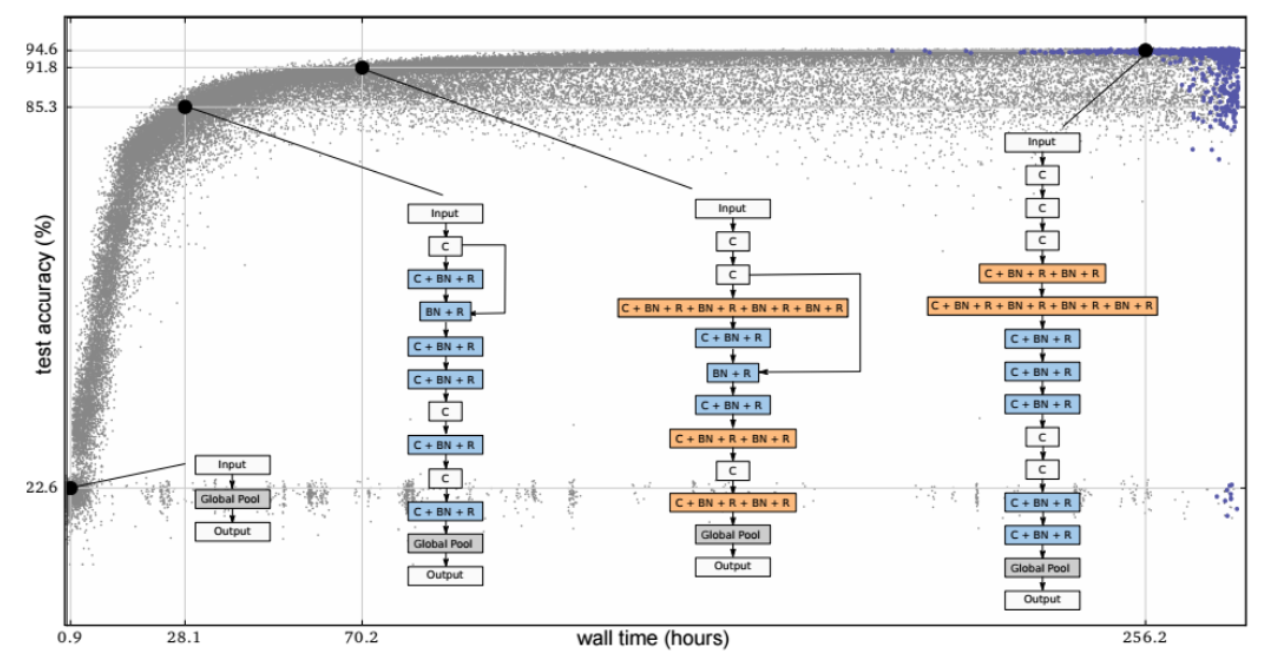
\includegraphics[width=\linewidth]{figures/nas.png}
  \caption{Neural architecture search become exponentially expensive with respect to marginal accuracy (Image credit: Towards Data Science, 2019)}
  \label{fig:nas}
\end{figure}





\section{Methods}
\label{sec:methods}
To test our hypothesis, we constructed a simple, two-layer recurrent neural network (based on Aungiers, 20184). For data, we used publically available pricing data from the AWS spot market. Effectiveness was measured by how well our network could predict the next spot price. 
We developed two workflows, one as a baseline and one as a test case (illustrated to the right). The RNN was constructed using Keras with a Tensorflow back-end and the workflows were completed using this implementation within a Python notebook. Each workflow was run 10 times in order to ensure accuracy and reproducibility.
The baseline workflow simply trains our neural network from N different initialization and then choses the trained model with the lowest loss after K epochs. This is effectively the same as retraining a number of times to find a trained model with the best parametrization.
Our experimental workflow begins in the same manner as the baseline workflow. However, during the training (for example, after K/2 epochs), optimization is halted and only the top T networks are selected. We then merge the weights of the two networks using some predefined function, an illustration of which is pictured to the right. We then re-spawn N networks with slight random mutations between them and continue training until we have reached K epochs.

\begin{figure}[h!]
\begin{subfigure}[h]{0.49\linewidth}
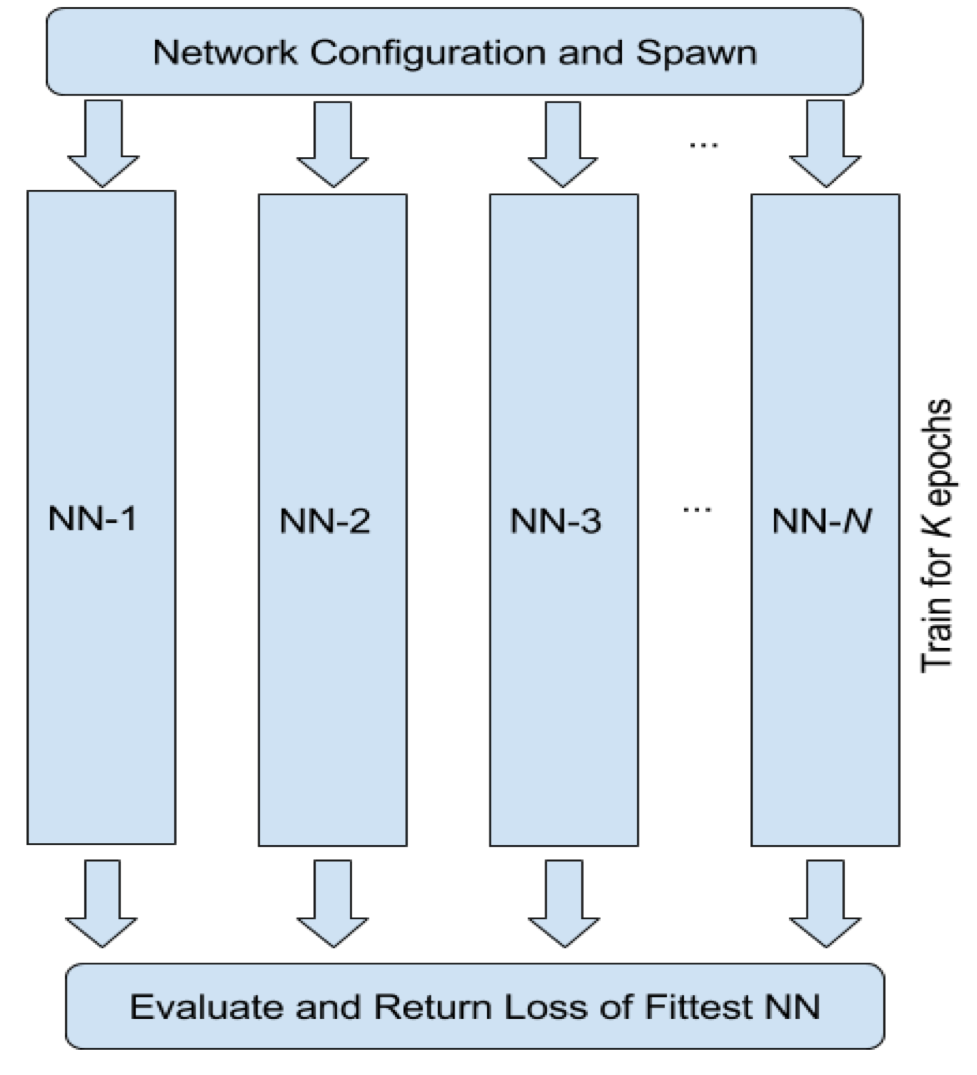
\includegraphics[width=\linewidth]{figures/simple.png}
\caption{Control, no cross-over.}
\end{subfigure}
\hfill
\begin{subfigure}[h]{0.49\linewidth}
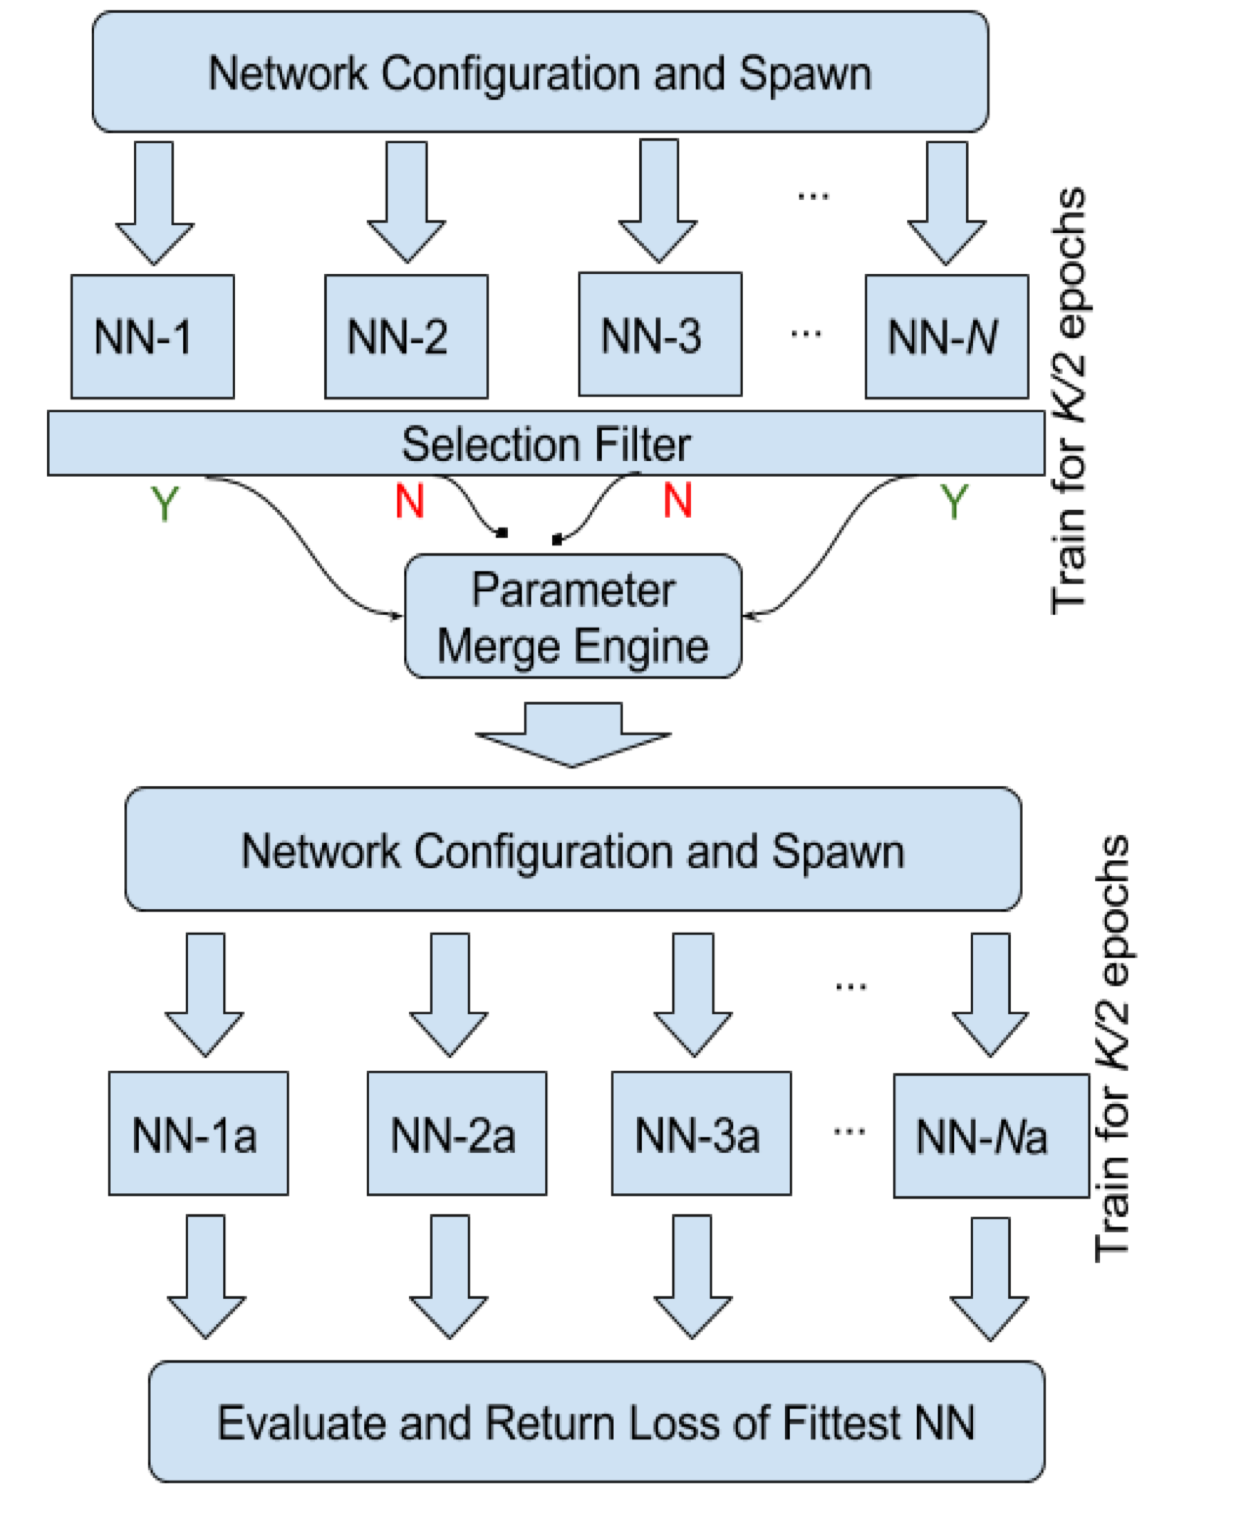
\includegraphics[width=\linewidth]{figures/workflow.png}
\caption{Test, with cross-over.}
\end{subfigure}%
\caption{Generalized control and test workflows used to evaluate parameter merging.}
\end{figure}

\begin{figure}[h!]
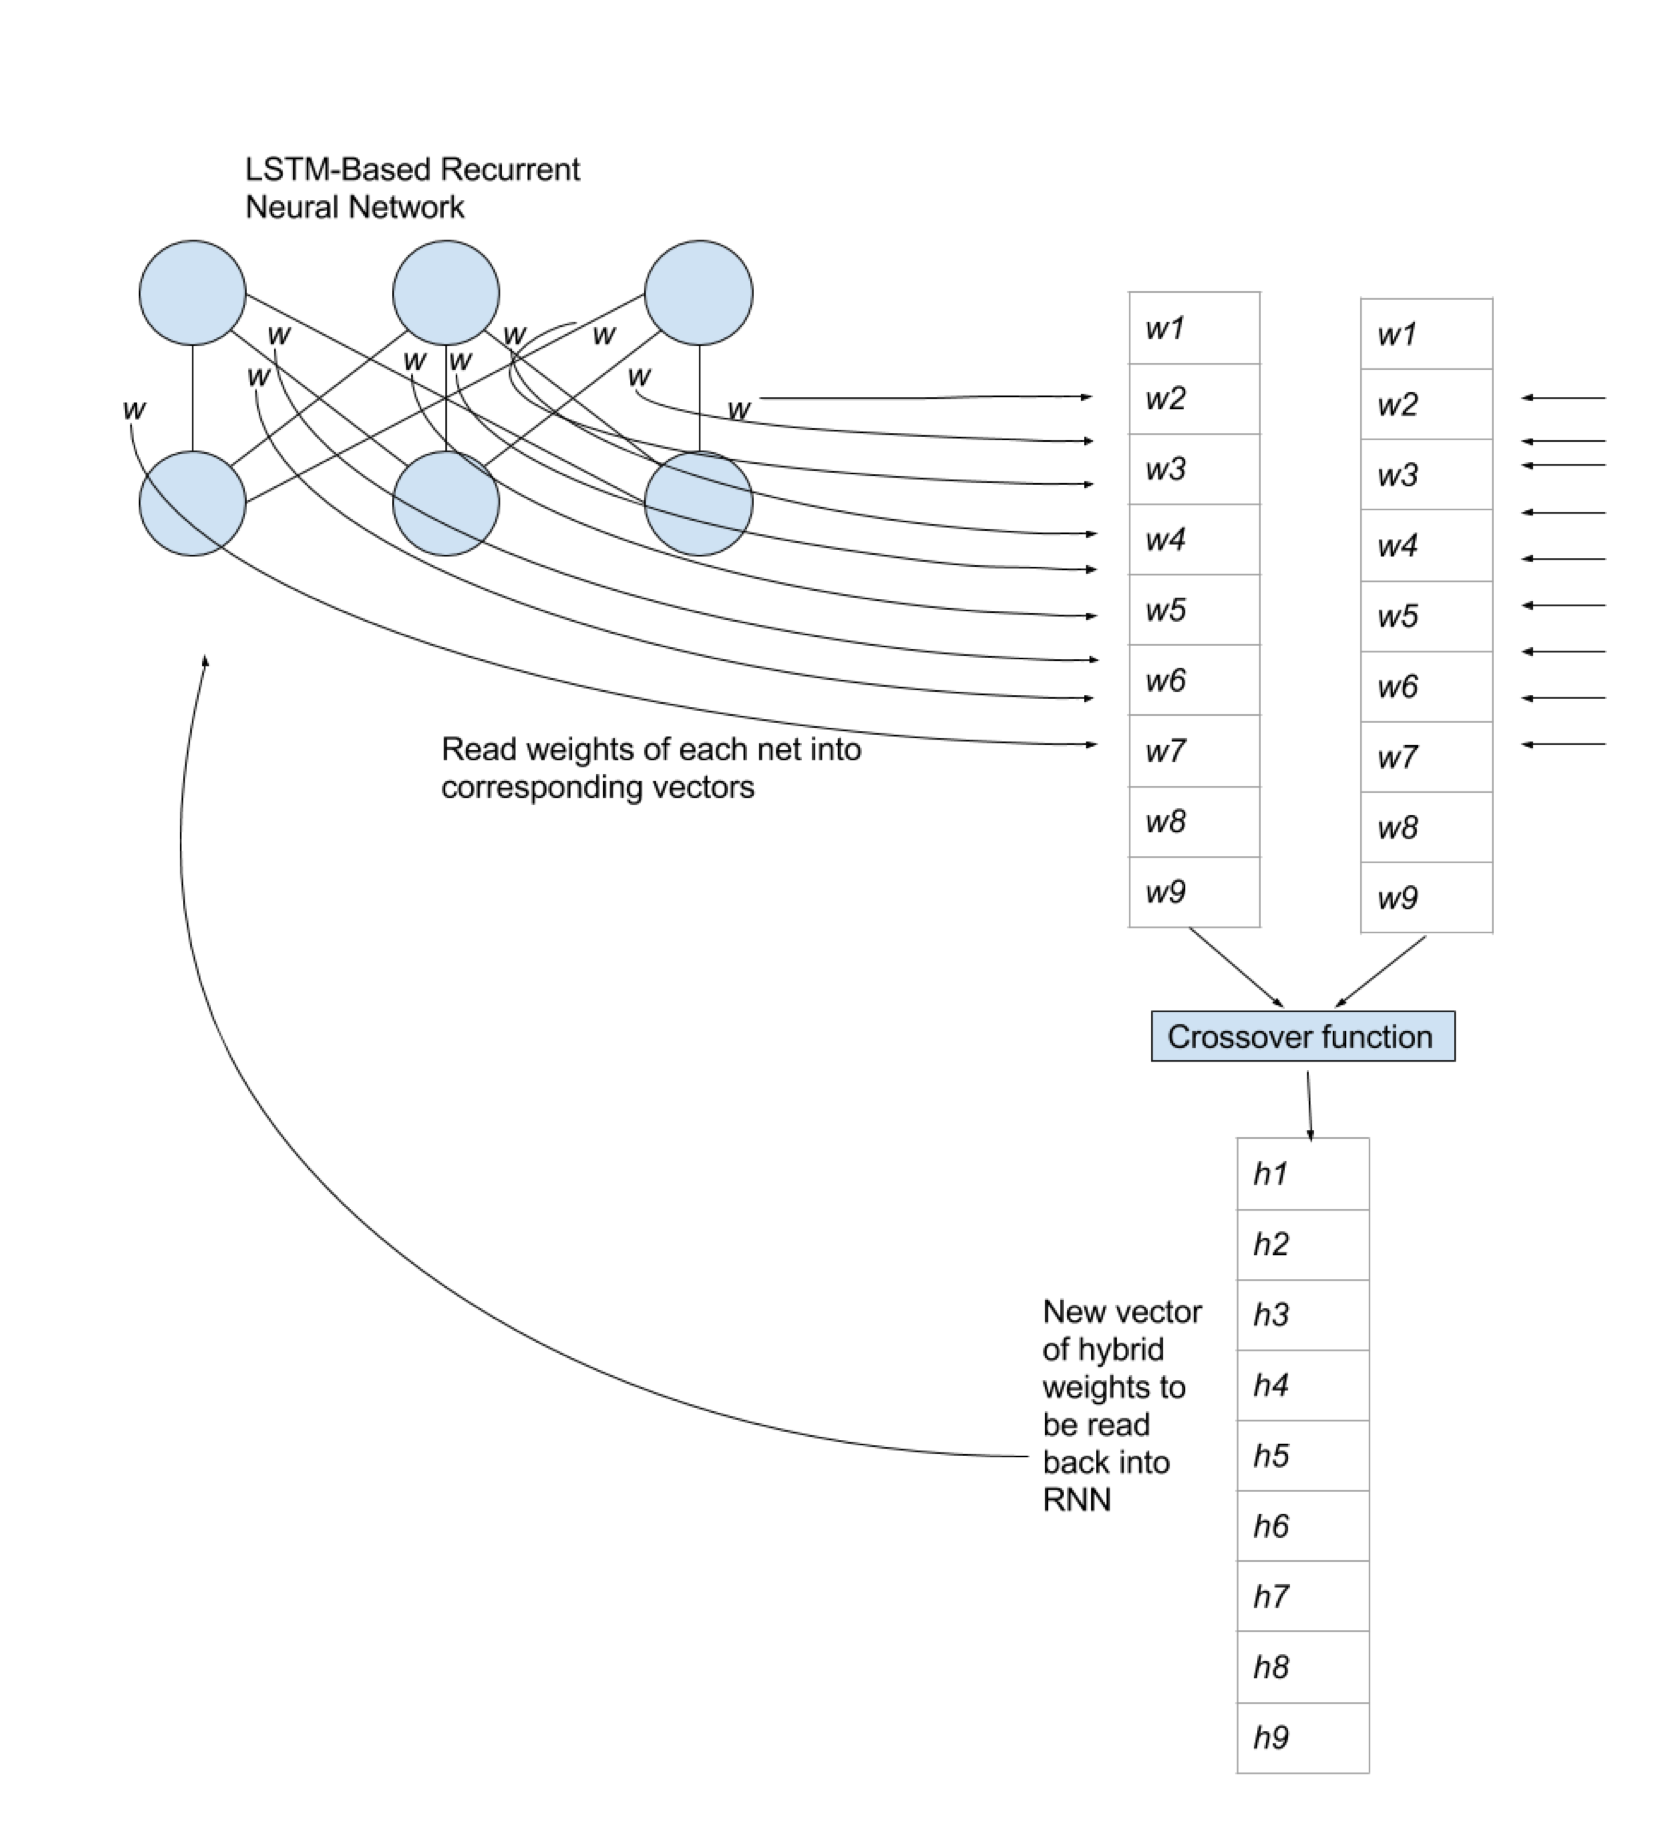
\includegraphics[width=\linewidth]{figures/merge.png}
\caption{Illustration of merging network weights}
\end{figure}
\section{Results}
\label{sec:results}

Statistical significance was achieved between our test case and our baseline regardless of whether we used random selection or parameter means. Between these two methods, taking the mean showed better accuracy, though not significantly so. Results varied between workflow runs but we observed differences in effect that increased the ending loss by as much as 5\% compared to the control and that decreased the ending loss as much as 20\%. 
There is little improvement after merging the networks following a short amount of time, however, there is significant improvement (including a quicker convergence) following a merge of two well-trained networks.
Though overall results were significant, we have observed bias in our testing towards partially trained models with similar parameter values. This aligns with our initial thoughts regarding the structure and shape of the parameter search space. Namely, for two local optima, it is not unlikely that another local optimum exists in a location between the two prior values.
\begin{figure}[h!]
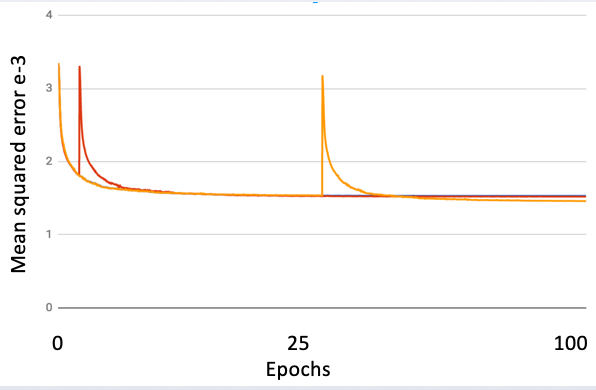
\includegraphics[width=\linewidth]{figures/loss.png}
\caption{Mean loss across 5 trial runs comparing the use of cross-over.}
\label{fig:results}
\end{figure}
\section{Conclusion}
\label{sec:conclusion}

The introduction of variation using fitness selection and crossover allows for quicker convergence and greater accuracy of certain neural networks. In our tests, we observed cases where little to no improvement was seen and we observed cases where error could be reduced  as much as 20\%. This seems to indicate dependence on initial condition and on specific network initializations and randomizations performed at the beginning of each workflow. In all, we have clearly presented a more efficient workflow for refining optimal parameterizations for neural networks compared to random retraining. Therefore, we have shown this methods viability to increase accuracy and reduce computation necessary for accurately training a RNN.





\section*{Acknowledgments}
We must thank the Illinois Institute of Technology and their BigDataX REU Program, as this was the source of funding for this research. We must also thank Argonne National Labs for hosting this research and for providing countless hours of compute time.

\ifCLASSOPTIONcaptionsoff
  \newpage
\fi
\nocite{*}
\bibliography{refs}
\bibliographystyle{ieeetr}



% that's all folks
\end{document}


